% DO NOT COMPILE THIS FILE DIRECTLY!
% This is included by the other .tex files.

\begin{frame}[t,plain]
\titlepage
\end{frame}




\begin{frame}[t]{Host a Probar}

\textbf{Creación de PATH}

\begin{wrapfigure}{r}{0.43\textwidth} 
\vspace{2pt}
  \begin{center}
    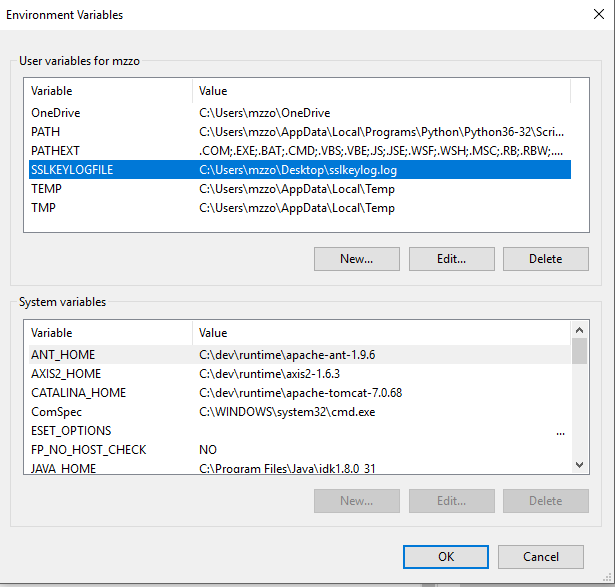
\includegraphics[width=0.45\textwidth]{sslpath.png}
    \label{fig:databaseUserTable}
  \end{center}
  \vspace{2pt}
\end{wrapfigure} 

\bigskip

Es necesario generar un nuevo PATH en las variables ambiente, declarando la dirección a apuntar y el archivo a generar, el cual será:

\begin{center}
   \textbf{sslkeylog.log}
\end{center}


\end{frame}



\begin{frame}[t,fragile]{Herramientas}

\textbf{El archivo obtenido}

\begin{wrapfigure}{r}{0.43\textwidth} 
\vspace{2pt}
  \begin{center}
    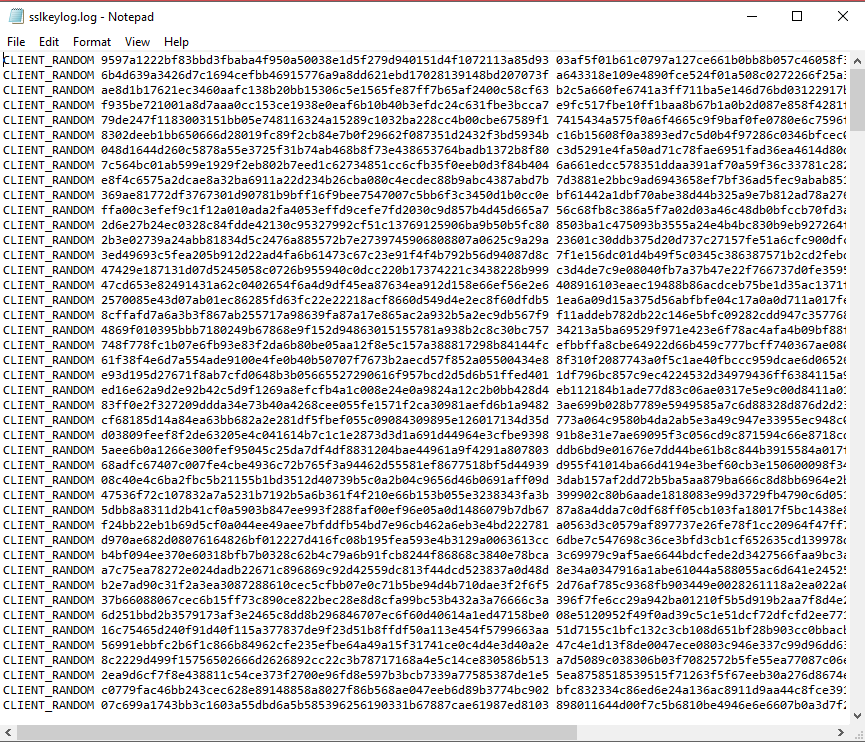
\includegraphics[width=0.45\textwidth]{ssllog.png}
    \label{fig:databaseUserTable}
  \end{center}
  \vspace{2pt}
\end{wrapfigure} 

\bigskip

Se aprecian los datos obtenidos en el archivo \textbf{sslkeylog.log}, donde se declara el cliente, llave y rsa.

\begin{center}
   
\end{center}

\end{frame}

\begin{frame}[t,fragile]{Herramientas}

\textbf{WireShark Implementación de Certificados}

\begin{wrapfigure}{r}{0.43\textwidth} 
\vspace{2pt}
  \begin{center}
    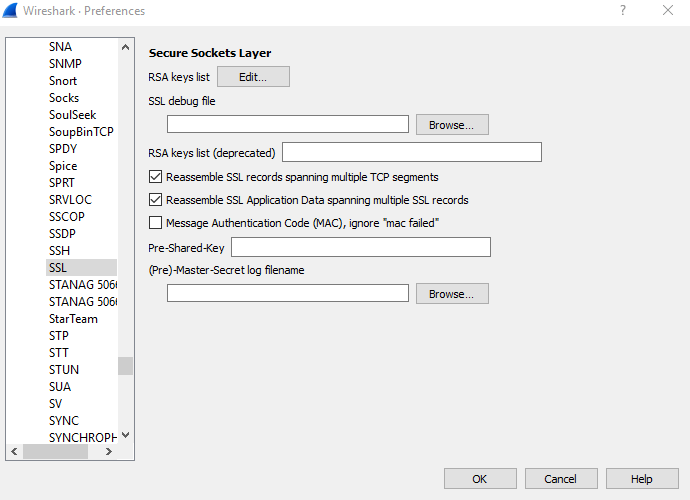
\includegraphics[width=0.45\textwidth]{wiressl.png}
    \label{fig:databaseUserTable}
  \end{center}
  \vspace{2pt}
\end{wrapfigure} 

\bigskip

Ya en previa emisión de internet por parte del computador, es necesario proveer los certificados generados, contal de ver la respuesta dentro de la aplicación.

\begin{center}
   
\end{center}

\end{frame}

\begin{frame}[t,fragile]{Herramientas}

\textbf{Búsqueda de Carpeta con Certificados }

\begin{wrapfigure}{r}{0.43\textwidth} 
\vspace{2pt}
  \begin{center}
    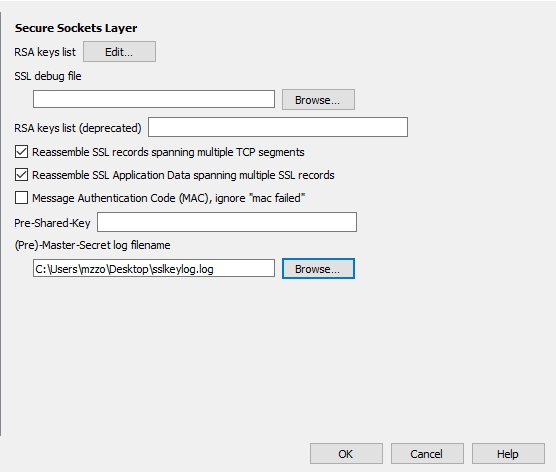
\includegraphics[width=0.45\textwidth]{archivossllog.png}
    \label{fig:databaseUserTable}
  \end{center}
  \vspace{2pt}
\end{wrapfigure} 

\bigskip

Es necesario proveer la ruta especifica en donde se encuentra el archivo generado por el PATH, de tal manera que trabajen como decifradores de las request generadas al hacer man-in-the-middle.
Se consigue la ruta especifica en donde se encuentra el archivo generado por el PATH, de tal manera que trabajen como decifradores de las request generadas al hacer man-in-the-middle.



\end{frame}



\begin{frame}[t,fragile]{Herramientas}

\textbf{Uso de Wireshark}

\begin{wrapfigure}{r}{0.43\textwidth} 
\vspace{2pt}
  \begin{center}
    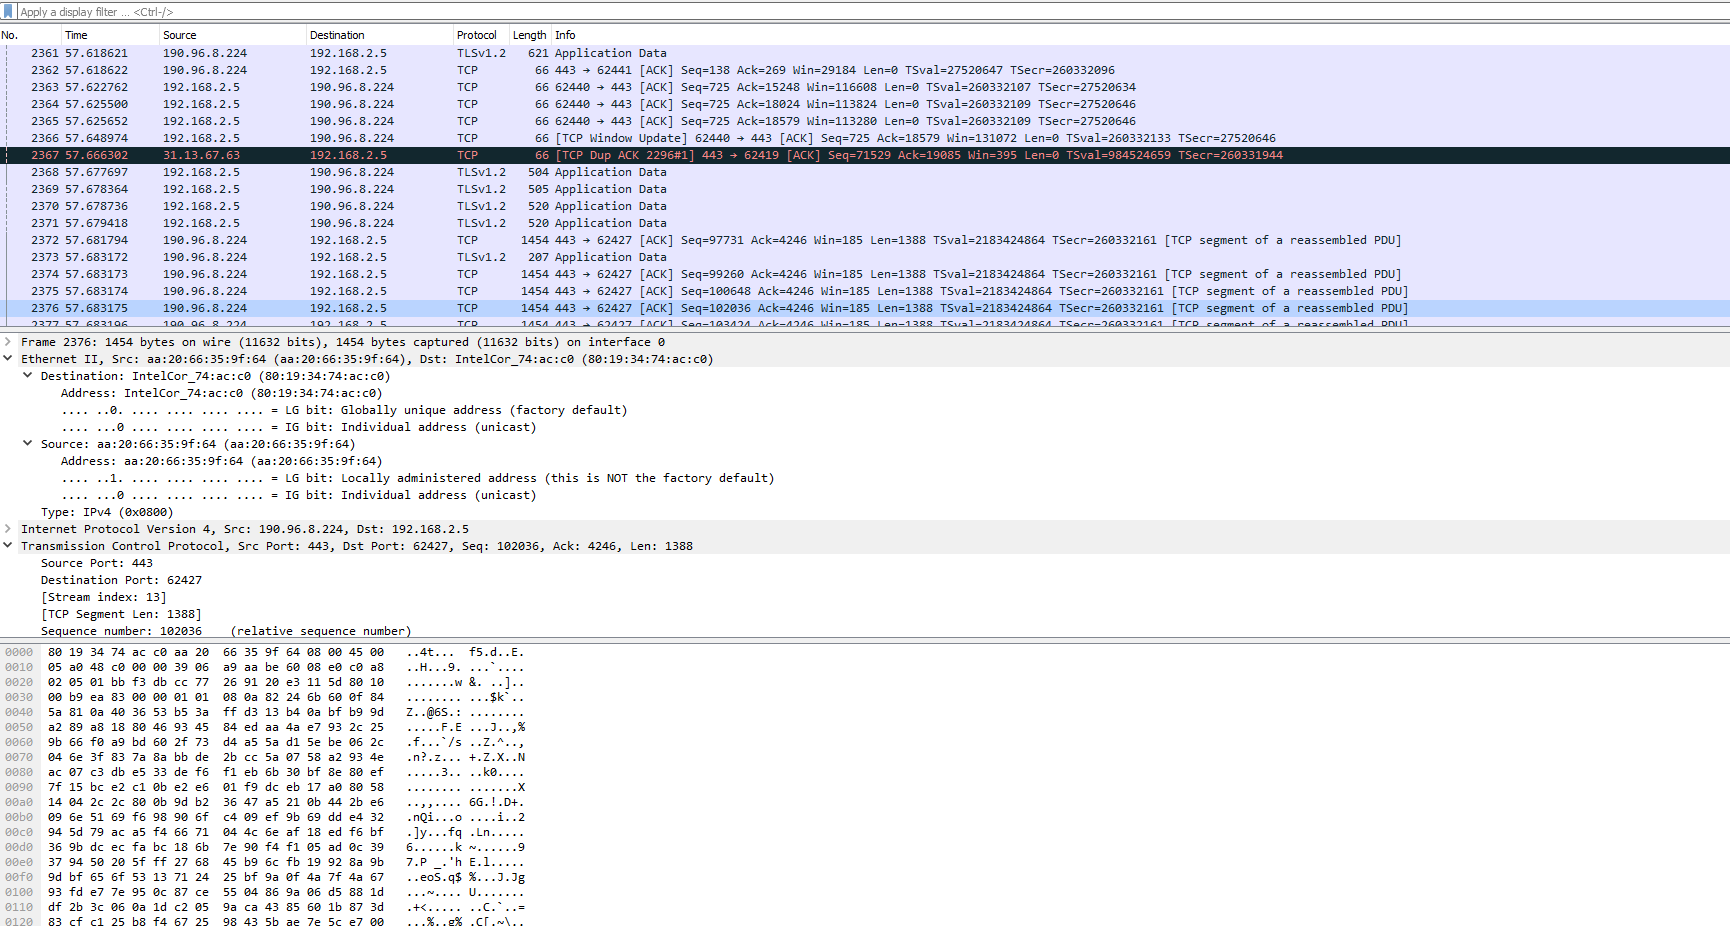
\includegraphics[width=0.45\textwidth]{paqueteswiressl.png}
    \label{fig:databaseUserTable}
  \end{center}
  \vspace{2pt}
\end{wrapfigure} 

\bigskip

Se adjunta las imagen correspondiente a los paquetes recibidos dentro de la aplicación haciendo uso del celular como emisor de paquetes, de entre los cuales se logra apreciar ciertos paquetes.


\end{frame}


\begin{frame}[t,fragile]{Herramientas}

\textbf{Uso de Wireshark}

\begin{wrapfigure}{r}{0.43\textwidth} 
\vspace{2pt}
  \begin{center}
    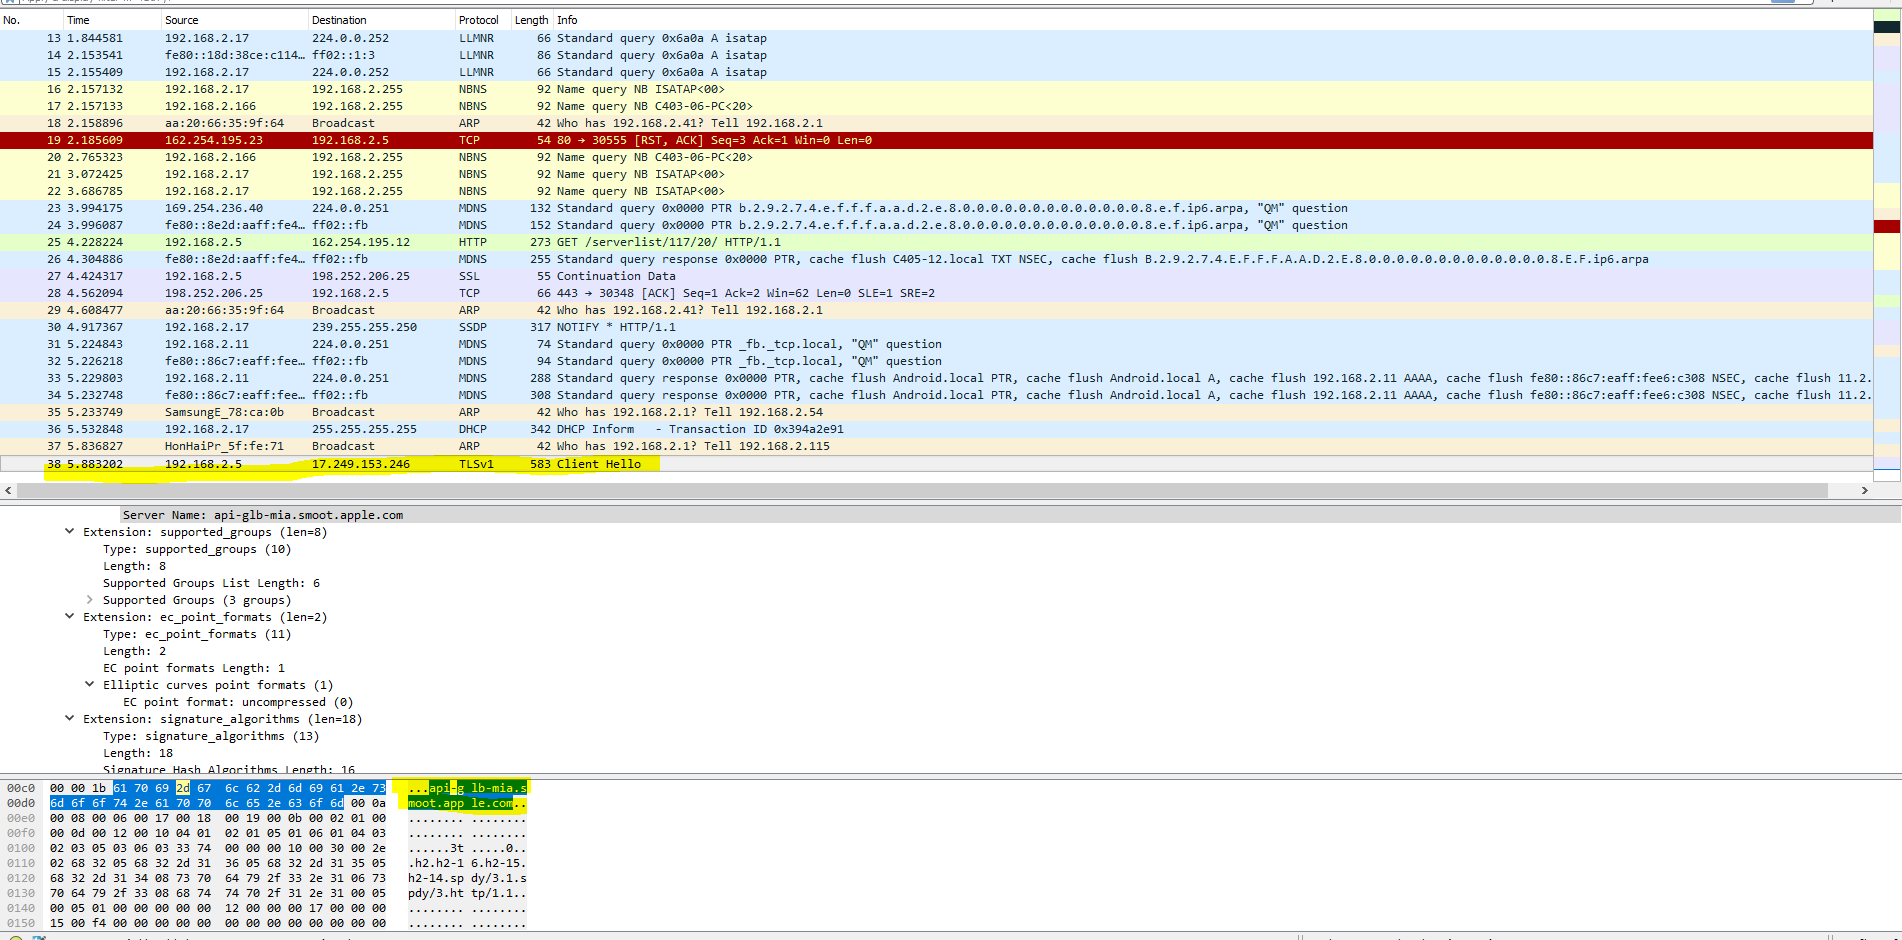
\includegraphics[width=0.45\textwidth]{paquetelectura.png}
    \label{fig:databaseUserTable}
  \end{center}
  \vspace{2pt}
\end{wrapfigure} 

\bigskip

Es posible apreciar lectura de los paquetes, entregando pauetes del tipo TCP y CLIENT HELLO, de la cuál se adjunta una recepción del paquete mayormente ilegible, pero aún así, no se encuentra información consistente y tangible de las respuestas. Lo que implica que no es posible captar la información de los usuarios o bien sentencias explotables.


\end{frame}